\begin{abstract}
Prompt caching bills tokens a provider has already seen at about a tenth of the list price, but only when a request starts with exactly the bytes of an earlier one. Agent builders therefore keep the context append-only: nothing is reordered and nothing is deleted. When a value changes, the old value stays in the context beside the new one. We test whether this layout costs accuracy, with the information content held fixed, and whether the cache discount pays for that cost. StaleTrap is a frozen testbed of 144 scripted tool-using episodes (720 questions, 2,376 tool calls). We replay each episode under four layouts that carry the same information: append-only, relevance-reordered, stale values redacted in place, and append-only plus a short note. Every call is billed and cache-metered by the provider. On Gemini 3.1 Flash-Lite, questions about the agent's own updates and neutral questions are answered perfectly under every layout. When the update came from outside the agent, append-only answers 65.5\% correctly, against 96.0\% with redaction, 70.5\% with reordering and 73.5\% with the note. Append-only is the cheapest layout per episode (1.05 against 1.16 cents), but redaction is the cheapest per correct episode (1.22 against 1.52 cents) at every cache-read price from free to full. Across three Gemini generations, append-only accuracy on these questions rises from 40\% to 66\% to 80\%, and its gap to redaction shrinks from 27 to 18 to 11 points without closing.
\end{abstract}

\section{Introduction}
\label{sec:intro}


Agent builders now design their prompts around the provider's cache. Providers bill input tokens they have already processed at about a tenth of the list price, and the discount applies only when a request starts with exactly the bytes of an earlier request \citep{a2312_07104,a2601_06007}. Practitioner guidance follows from this: put the system prompt and tools first and never change them, append every new observation at the end, and never reorder or delete earlier blocks \citep{manus2025,anthropic2025context}. We call this the \emph{cache-optimal layout}.

\begin{figure}[t]
\centering
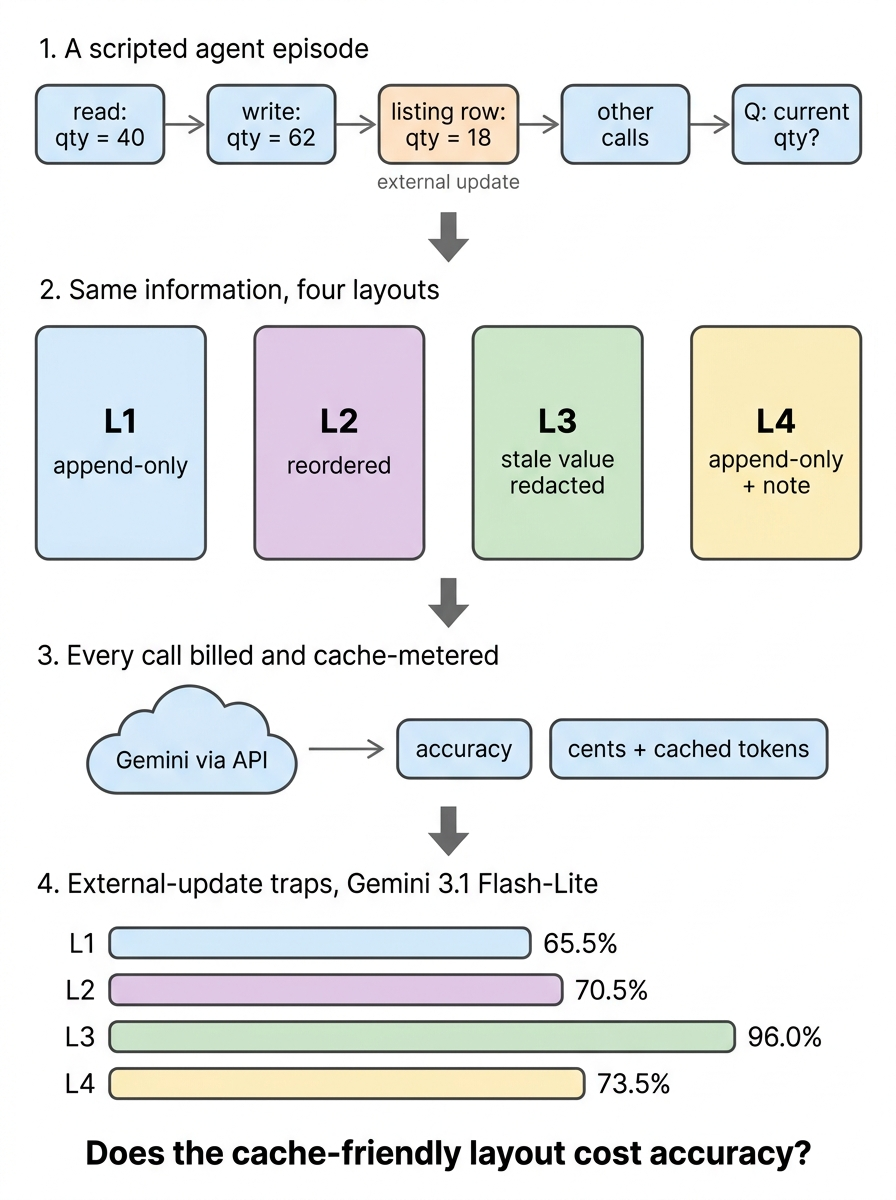
\includegraphics[width=0.75\columnwidth]{assets/fig1_schematic.png}
\caption{Study design. A scripted agent episode (the values shown are an example) is replayed under four layouts that carry the same information. Every call goes to the provider's API, which reports billed cost and cached tokens. The bars give accuracy on external-update questions for Gemini 3.1 Flash-Lite.}
\label{fig:schematic}
\end{figure}

This layout has a cost that the guidance does not price. Because nothing is removed, an old value stays in the context next to its replacement, and the model must pick the later one. Prior work shows this is hard: the latest of several revisions of a fact is retrieved less reliably as revisions accumulate \citep{a2603_12271,a2510_22752}, and agents answer from observations the world has overtaken \citep{a2610_05281}. Two literatures sit on either side of the question. Context-management papers prune old observations and report accuracy, but price tokens at list rates with no cache discount \citep{a2606_10209,a2508_21433,a2605_18854}. Caching papers report cost and latency but not accuracy \citep{a2601_06007,a2607_15516}. Nobody has measured whether the cache-optimal layout itself, with the information held fixed, costs accuracy, or what that cost is worth against the cache discount.

We measure both with a controlled replay (Figure~\ref{fig:schematic}). In StaleTrap, a deterministic tool environment, we know by construction whether each question has an outdated value in the context, and whether the update came from the agent's own write or from an outside change that appears only as one row of a listing. We replay each episode under four layouts with the same information and record the provider's bill and cached tokens for every call.

Our contributions are:
\begin{itemize}
\item \textbf{StaleTrap}, a frozen testbed of 144 scripted tool-using episodes in which every question is labelled as a stale-value trap (own or external update) or a neutral question.
\item \textbf{A layout experiment that holds content fixed} and scores accuracy against provider-billed cost and cached tokens.
\item \textbf{The finding that the accuracy cost is confined to external updates}: zero on own updates and neutral questions, 30.5 points on external updates for Gemini 3.1 Flash-Lite.
\item \textbf{The finding that redaction is cheaper per correct episode at every cache-read price} on the tested models, because the provider's cache rarely serves the history under any layout.
\end{itemize}

\section{Related Work}
\label{sec:related}

\paragraph{Position and stale values.} Models use the start and end of a long context better than its middle \citep{a2307_03172,a2406_16008}. Repeated keys are retrieved at their first and last occurrence \citep{a2510_22752}, and the latest of several revisions is retrieved less reliably as revisions accumulate \citep{a2603_12271}. Reordering passages by relevance is no better than shuffling in realistic retrieval \citep{a2505_15561}. In agents, observations go stale \citep{a2610_05281}, masking old observations helps mid-capacity models only \citep{a2606_00408}, and time stamps alone do not tell a model which version is current \citep{a2602_01313}.

\paragraph{Prompt caching.} Exact-prefix reuse is the production default \citep{a2312_07104,a2311_04934}. Caching cuts the cost of long agent sessions by 40 to 80 percent, and the discount is lost when earlier bytes change \citep{a2601_06007,a2607_15516}. Production hit rates are near 90 percent within a turn and 55 percent across turns \citep{a2608_00101}. The closest work measures provider-billed cost, split into cache creation and reads, against task success, and shows that compressing tool outputs can raise the bill by changing trajectories \citep{a2607_12161}; it varies compression, which changes content, not layout.

\paragraph{Context management and cost-aware evaluation.} Pruning history to the last few tool pairs raises completion and cuts tokens \citep{a2606_10209}, and observation masking matches LLM summaries at a fraction of the cost \citep{a2508_21433,a2605_18854}. Cost-controlled evaluation asks for an accuracy-against-dollars frontier \citep{a2407_01502,a2504_13359,a2510_11977}. None of these isolates layout from content, and none includes the cache discount in the cost. Table~\ref{tab:delineation} in the appendix compares our design with each close neighbour.

\section{Experimental Setup}
\label{sec:setup}

\paragraph{Why a purpose-built testbed.} To attribute an error to a stale value, we must know, for every question the agent answers, whether a superseded value for the queried field is in its context. Public agent benchmarks do not annotate this, so we built StaleTrap, a deterministic tool environment in which the annotation is known by construction. The testbed was frozen with a recorded hash before any scored run.

\paragraph{Environment.} Three back-office domains (warehouse inventory, a shared meeting calendar, a support-ticket queue) are exposed as 29 JSON-schema tools: 10 reads and 19 writes. A fourth domain of 10 messaging and HR tools is present in every call and never needed, so the catalogue is masked by the agent's choice rather than trimmed per step, as production stacks do. A local executor holds the state and returns realistic JSON. Every result declares which (record, field) values it states: a read states the fields it returns, a write states the field it changed and its new value, and a listing states every row it contains. The fixed prefix (system prompt and tool declarations) is 5,102 tokens on Google's tokenizer, above every provider's minimum for implicit caching.

\paragraph{Episodes.} An episode is a scripted sequence of user instructions. Most ask for one tool call (``Record that we received 22 units of SKU-2249''). Some are questions answered from the context with tools disabled, returned as a one-key JSON object and scored by exact match against the executor's live state. A \textbf{trap thread} reads a field, updates it one to three times, and then asks for its current value, so an outdated value is in context. A \textbf{neutral thread} reads a field once and asks for it later. In an \emph{own} update the agent's own write returns the new value. In an \emph{external} update someone else changes the record, and the agent sees the new value only as one row of an unrelated listing it was asked to fetch, which is the realistic source of stale observations \citep{a2610_05281}. Five of nine task templates use external updates and four use own updates. The remaining calls are distractors: compact reads and writes on unrelated records at the \emph{low} level, and verbose listings, near-miss identifiers and writes to other fields of the queried records at the \emph{high} level. Episodes have 6, 12, 18 or 30 tool calls with 2 to 8 questions, and the distance from the last update to its question grows with length. The grid crosses 3 domains, 3 templates, 4 lengths, 2 distractor levels and 2 seeds: 144 episodes, 720 questions (360 trap, 360 neutral) and 2,376 tool calls. A script checks that every stale value differs from the final answer (360 of 360), and every task has a second phrasing for a robustness check.

\paragraph{Layouts.} Each turn, the runner rebuilds the message list under one of four rules. \textbf{L1} is the cache-optimal layout: every block in arrival order. \textbf{L2} keeps the same blocks but sorts earlier ones by relevance to the current turn, so the prefix changes every turn. \textbf{L3} keeps arrival order but replaces every value that a later result restated with ``\textless superseded at step $k$\textgreater''. L3 uses the executor's schema, so it is an upper bound for any real pruner, and it breaks the cached prefix at the first edit. \textbf{L4} is L1 plus a short note added to every user turn and kept there, so the history stays append-only. The note gives the session goal, the step number and, for every record observed more than once, which step is current and which steps are superseded. It never contains a value, so it cannot leak an answer. It adds about 150 tokens per turn, and because earlier notes stay in the history an L4 episode sends more prompt tokens than an L1 episode. L1, L2 and L4 carry identical information; the appendix shows one episode serialised under each layout.

\paragraph{Models.} Table~\ref{tab:models} lists the three Gemini models, all called through OpenRouter at temperature 0 with minimal reasoning effort. We planned three model families, but a guardrail on the API account blocked every non-Google model, so the study is a three-generation Gemini ladder. Gemini 3.5 Flash-Lite was dropped because about a third of its tool calls were malformed. Calls use a per-episode session identifier for sticky routing, and turns run strictly in sequence so that the cache never expires between turns. Caching on Google is implicit; an explicit breakpoint on Gemini creates a billed cache on every call, which we measured at 3.5 to 5.8 times the cost of an implicit hit. Every call logs the provider's prompt, cached and completion tokens and the billed amount; no cost in this paper is estimated from a price sheet except where we say counterfactual.

\begin{table}[t]
\centering\small
\setlength{\tabcolsep}{4pt}
\begin{tabular}{@{}lrlr@{}}
\toprule
Model & Tasks & Layouts & Episodes \\
\midrule
Gemini 2.5 Flash & 72 & L1, L3, L4 & 216 \\
Gemini 3.1 Flash-Lite & 144 & L1--L4 & 576 \\
Gemini 3.6 Flash & 36 & L1, L3 & 72 \\
\bottomrule
\end{tabular}
\caption{Models and runs. Gemini 3.1 Flash-Lite runs the full grid; Gemini 2.5 Flash (older, thinking on) runs the seed-0 half; Gemini 3.6 Flash (newest) runs a 36-task balanced subset.}
\label{tab:models}
\end{table}

\paragraph{Analysis.} The unit is the task. For each model we take within-task paired differences between layouts in trap accuracy, neutral accuracy, episode success (all questions right), billed cost and cached share of prompt tokens. We report two-sided sign-flip permutation tests over tasks with 20,000 flips \citep{good2005permutation} and task-bootstrap 95\% intervals with 10,000 resamples \citep{efron1994bootstrap}. Benjamini--Hochberg correction runs over the whole family of 65 tests \citep{benjamini1995bh}; 29 survive at $q = 0.05$. Following cost-controlled evaluation \citep{a2407_01502}, our cost metric is the billed cost per correct episode,
\begin{equation}
C_{\text{correct}} = \frac{\sum_e \mathrm{cost}(e)}{\sum_e \mathrm{success}(e)},
\label{eq:cpc}
\end{equation}
which we also recompute with every cached token repriced at 0 to 1 times the input price. Interactions (the trap gap by length, by distractor level, trap against neutral, and by model) are tested by label permutation. We hand-coded 40 wrong answers by error type, and two sensitivity checks guard the main contrast: accuracy restricted to questions whose scripted thread steps the agent actually executed, and accuracy on turns served from cache against turns that were not, at identical bytes.

\paragraph{Pre-registration.} Five directional predictions were logged before the first model call (verbatim in the appendix). \textbf{D1}: L1 is below L3 on traps, the gap grows with length, and there is no gap on neutral questions. \textbf{D2}: reordering does not beat L1 but costs much more. \textbf{D3}: the note recovers at least half of the L1-to-L3 gap while keeping L1's cache share, and sits on the frontier. \textbf{D4}: the gap shrinks with model capability. \textbf{D5}: there is a cache-read price below which append-only becomes the cheapest layout per correct task.

\section{Results}
\label{sec:results}

\begin{table*}[t]
\centering\small
\setlength{\tabcolsep}{4pt}
\begin{tabular}{@{}llcccccc@{}}
\toprule
Model & Layout & Trap acc. [95\% CI] & External trap & Success & Cents/episode & Cents/correct & Cached share \\
\midrule
Gemini 2.5 Flash & L1 append-only & 0.660 [0.565, 0.751] & 0.40 & 0.528 & \textbf{1.43} & 2.71 & \textbf{0.716} \\
 & L3 redacted & \textbf{0.933} [0.889, 0.971] & \textbf{0.84} & \textbf{0.861} & 1.54 & \textbf{1.78} & 0.710 \\
 & L4 note & 0.875 [0.811, 0.932] & 0.75 & 0.778 & 2.45 & 3.15 & 0.683 \\
\midrule
Gemini 3.1 Flash-Lite & L1 append-only & 0.806 [0.752, 0.857] & 0.655 & 0.694 & \textbf{1.05} & 1.52 & 0.708 \\
 & L2 reordered & 0.841 [0.792, 0.887] & 0.705 & 0.729 & 1.35 & 1.85 & 0.619 \\
 & L3 redacted & \textbf{0.983} [0.969, 0.994] & \textbf{0.960} & \textbf{0.944} & 1.16 & \textbf{1.22} & 0.676 \\
 & L4 note & 0.879 [0.837, 0.917] & 0.735 & 0.771 & 1.60 & 2.07 & \textbf{0.711} \\
\midrule
Gemini 3.6 Flash & L1 append-only & 0.889 [0.787, 0.972] & 0.80 & 0.833 & \textbf{3.51} & 4.21 & \textbf{0.475} \\
 & L3 redacted & \textbf{1.000} [1.000, 1.000] & \textbf{1.00} & \textbf{0.972} & 3.57 & \textbf{3.67} & 0.464 \\
\bottomrule
\end{tabular}
\caption{Per-layout results. Trap accuracy is the per-episode mean over all stale-value traps with a task-bootstrap 95\% interval; external trap is accuracy on external-update traps only (own-update traps and neutral questions are at or near 1.00 everywhere: neutral accuracy is 1.000 in every cell except Gemini 3.6 Flash L3, 0.972). Cost is provider-billed. \textbf{Bold}: best layout per model in each column.}
\label{tab:main}
\end{table*}

\paragraph{The accuracy cost is confined to external updates.} Table~\ref{tab:main} gives the per-layout results. On Gemini 3.1 Flash-Lite, L1 answers 80.6\% of trap questions and L3 answers 98.3\%. The paired difference is $-0.177$ [$-0.230$, $-0.128$], $p < 10^{-4}$, and survives correction (Table~\ref{tab:contrasts}). Neutral questions are answered perfectly under every layout. Splitting traps by kind locates the whole effect (Figure~\ref{fig:stale}). The 160 own-update traps are answered perfectly under every layout. On the 200 external-update traps, L1 scores 65.5\%, L2 70.5\%, L3 96.0\% and L4 73.5\%. When the agent's own tool reply states the current value, the old copy does no harm. When the current value arrived as one row of a listing fetched for another reason, the append-only agent answers from its own earlier write about one time in three. The gap does not grow with episode length: it is $-0.22$ at six calls and $-0.22$ at thirty (slope $+0.0006$ per call, $p = 0.85$), and does not depend on the distractor level ($p = 0.54$).

\begin{figure*}[t]
\centering
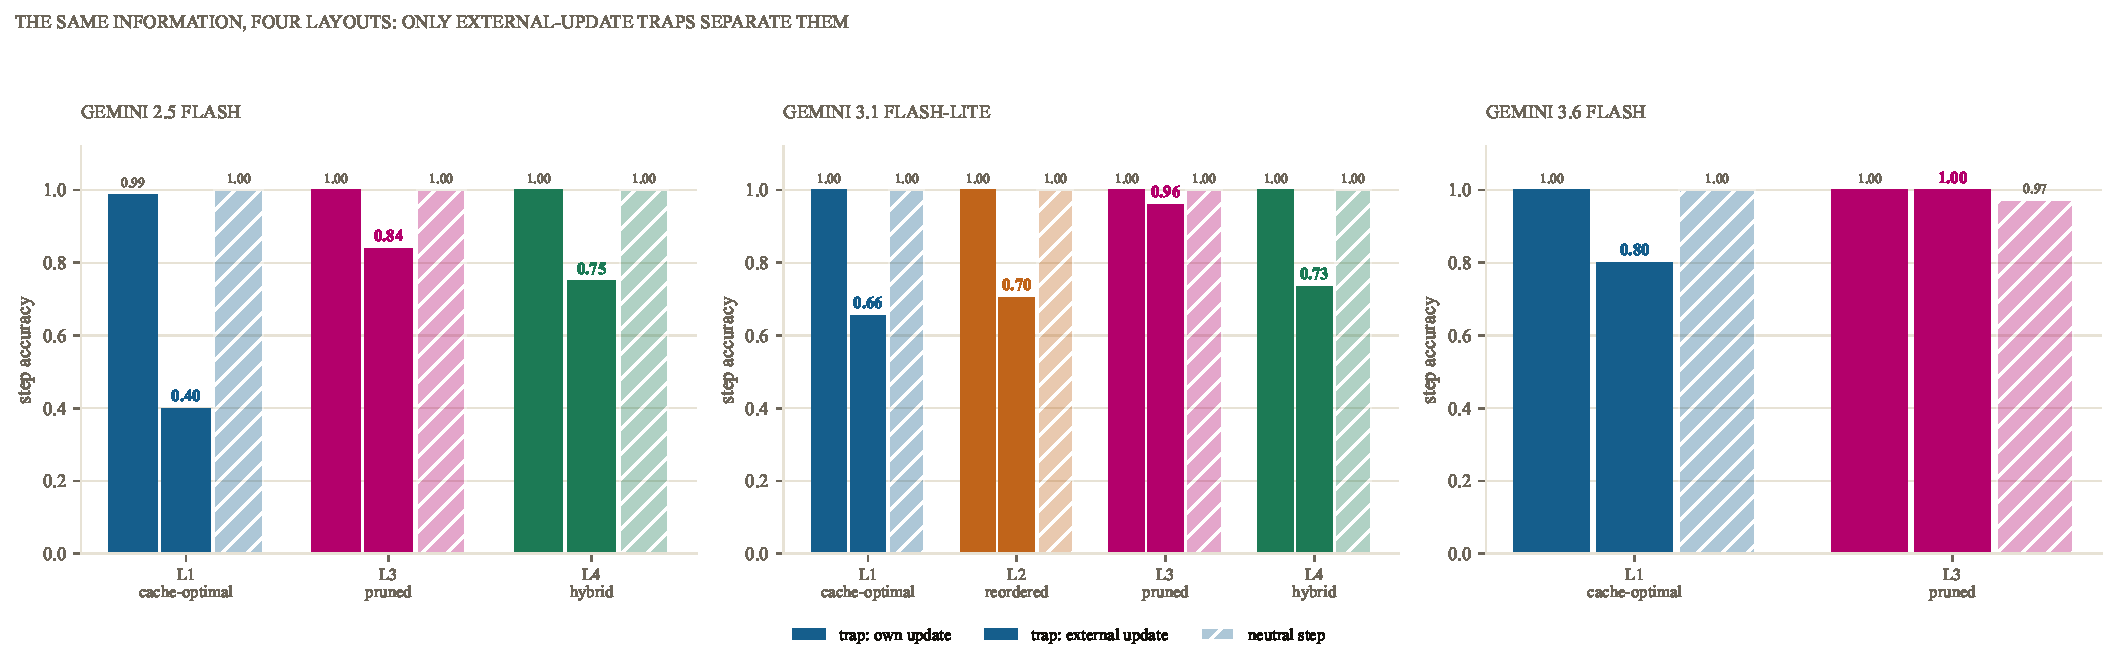
\includegraphics[width=0.9\textwidth]{assets/fig2_stale.pdf}
\caption{Question accuracy by layout on own-update traps, external-update traps and neutral questions, per model. Only the external-update bars move.}
\label{fig:stale}
\end{figure*}

\begin{table}[t]
\centering\small
\setlength{\tabcolsep}{3pt}
\begin{tabular}{@{}lcc@{}}
\toprule
Contrast & Trap acc. [95\% CI] & Cents/episode \\
\midrule
L1 $-$ L2 (order) & $-$0.036 [$-$0.079, 0.006] & \textbf{$-$0.30} \\
L1 $-$ L3 (content) & \textbf{$-$0.177} [$-$0.230, $-$0.128] & \textbf{$-$0.10} \\
L4 $-$ L1 (note) & \textbf{+0.073} [0.031, 0.120] & \textbf{+0.54} \\
L4 $-$ L3 & \textbf{$-$0.104} [$-$0.145, $-$0.066] & \textbf{+0.44} \\
\bottomrule
\end{tabular}
\caption{Paired within-task contrasts, Gemini 3.1 Flash-Lite (144 tasks). \textbf{Bold}: survives Benjamini--Hochberg correction. Every contrast and test is in the appendix.}
\label{tab:contrasts}
\end{table}

\paragraph{Reordering does nothing; the note recovers a quarter.} Reordering by relevance (L2) does not improve on L1 ($-0.036$, $p = 0.11$), and it rewrites the prefix every turn. The note (L4) improves on L1 by $+0.073$ ($p = 0.001$), which is 42\% of the L1-to-L3 gap over all traps and 26\% on external traps, while keeping L1's cached share. L4 remains well below L3 ($-0.104$, $p < 10^{-4}$).

\paragraph{What the wrong answers are.} Of 40 hand-coded wrong trap answers, 34 are an outdated value read back, almost always the agent's own earlier write, with the newer listing row ignored. Three are threshold questions where a stale read and a misread inequality coincide, two are cases where the agent skipped the listing call so the new value never reached its context, and one is a derived number. The agent executed the reveal steps 99.0\% to 100\% of the time under every layout, and restricting to fully executed threads moves no layout's accuracy by more than half a point.

\paragraph{The cheapest layout per episode is not the cheapest per correct episode.} L1 is the cheapest layout per episode at 1.05 cents; L3 costs 1.16 cents (paired $+0.10$ cents, $p < 10^{-4}$). Per correct episode (Eq.~\ref{eq:cpc}) the order reverses: L3 1.22 cents, L1 1.52, L2 1.85, L4 2.07. L1 and L3 are the only points on the accuracy-cost frontier (Figure~\ref{fig:frontier}). Repricing every cached token from free to the full input price (Figure~\ref{fig:threshold}) never changes the ranking: L3 is cheapest per correct episode at every price. On this provider no cache-read price makes the cache-optimal layout pay for its errors.

\begin{figure*}[t]
\centering
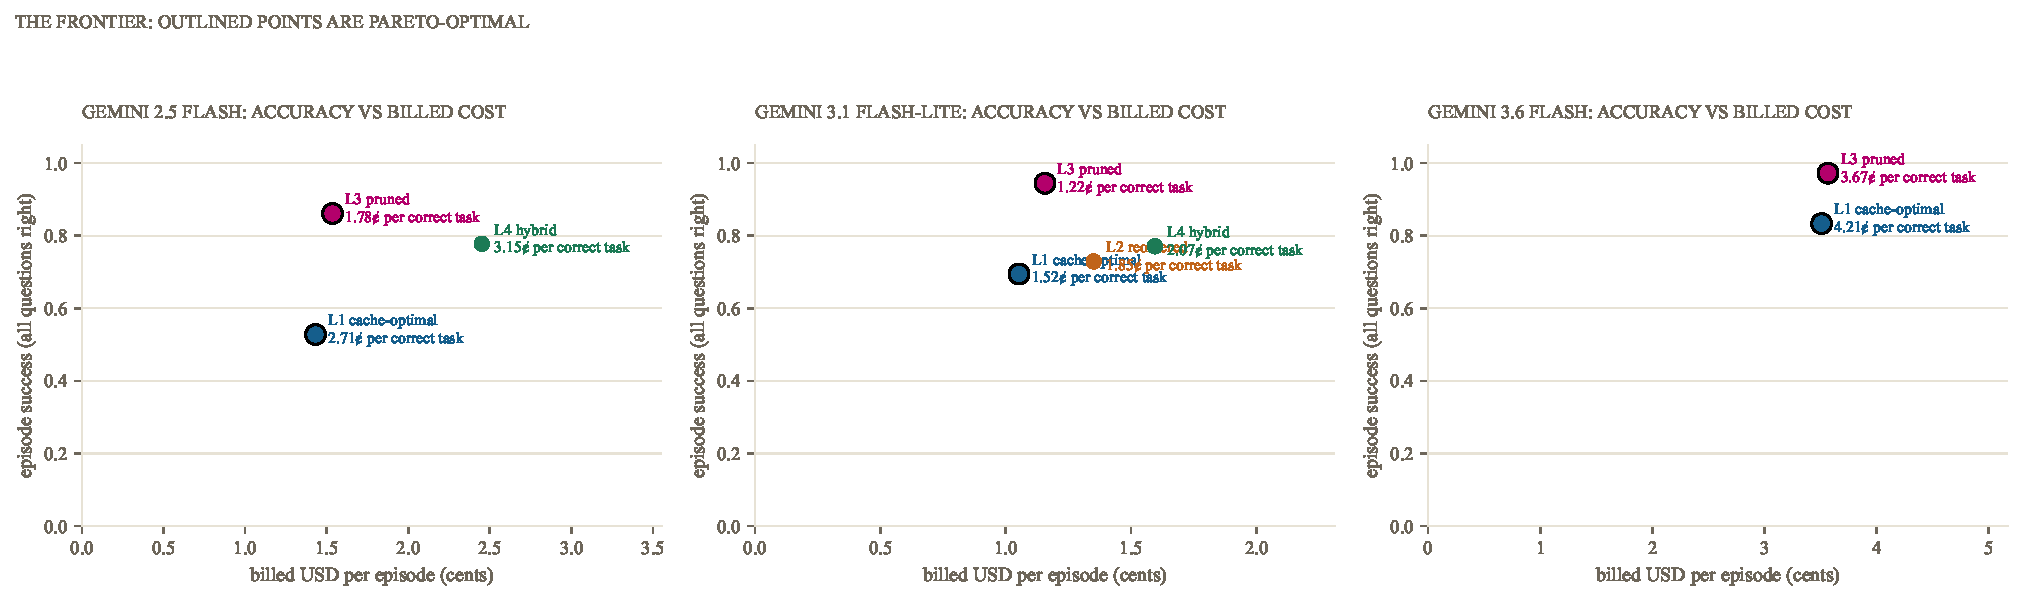
\includegraphics[width=0.8\textwidth]{assets/fig3_frontier.pdf}
\caption{Episode success against billed cents per episode, per model. Outlined points are on the frontier; cents per correct episode are annotated.}
\label{fig:frontier}
\end{figure*}

\begin{figure*}[t]
\centering
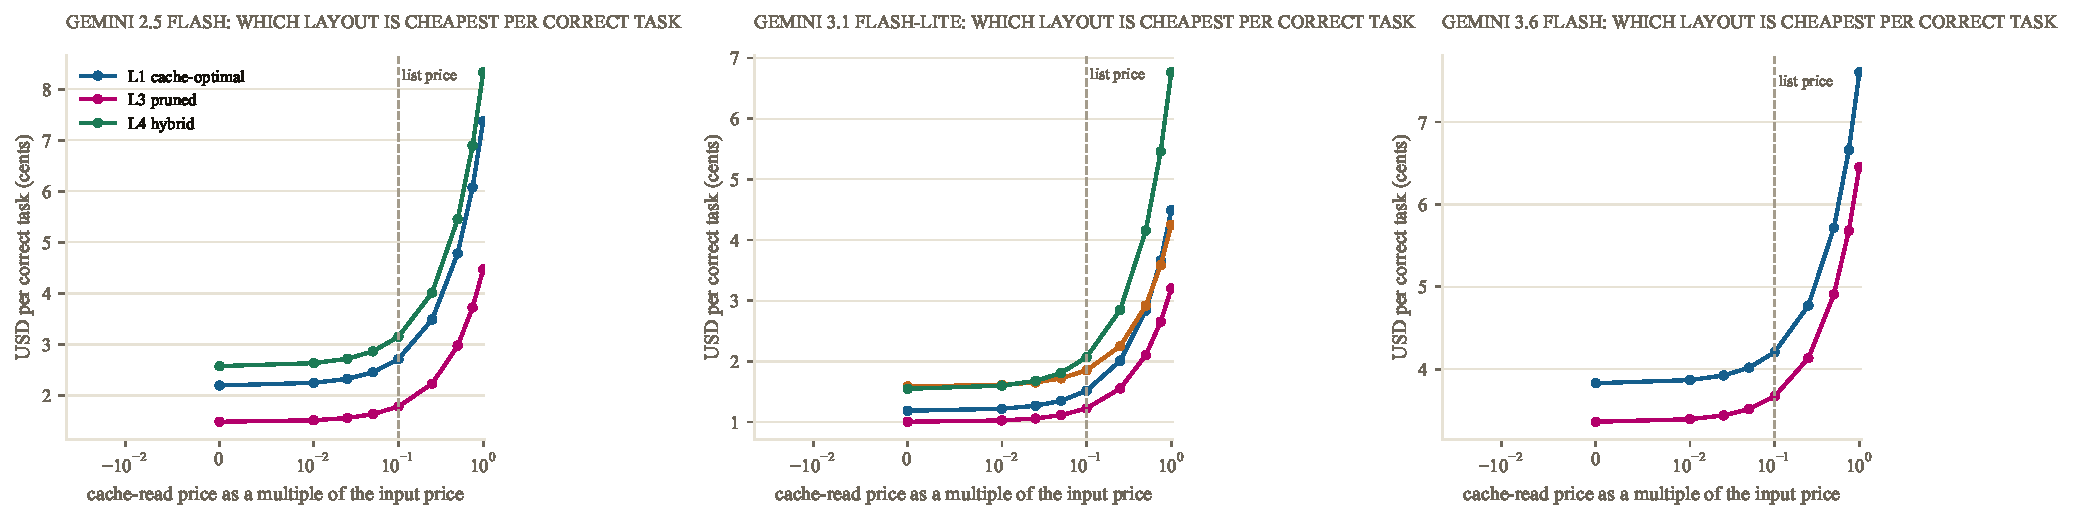
\includegraphics[width=0.8\textwidth]{assets/fig6_threshold.pdf}
\caption{Cents per correct episode under counterfactual cache-read prices from free (0$\times$) to the full input price (1$\times$). The billed point is 0.1$\times$. L3 is cheapest throughout.}
\label{fig:threshold}
\end{figure*}

\begin{figure*}[t]
\centering
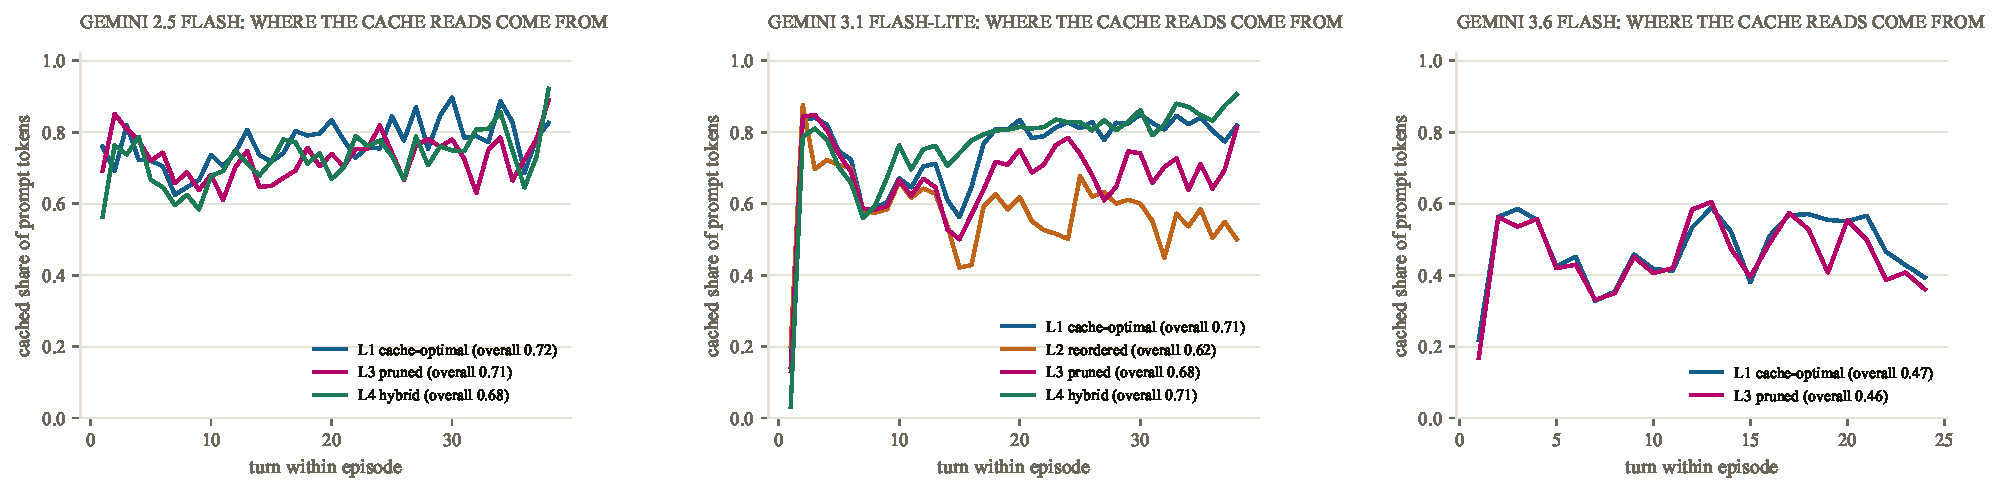
\includegraphics[width=0.72\textwidth]{assets/fig5_cache.pdf}
\caption{Cached-token share of the prompt by turn index, per layout, Gemini 3.1 Flash-Lite. The static prefix is cached from turn two under every layout; the history is cached on a minority of turns.}
\label{fig:cache}
\end{figure*}

\paragraph{Why: the history is rarely cached.} Figure~\ref{fig:cache} shows the cached share of prompt tokens by turn. Over an episode, the cached share of prompt tokens is 0.71 under L1 and 0.68 under L3, but most of that is the 5,100-token fixed prefix. Counting only the history, the cached share is 0.24 under L1, 0.13 under L2, 0.15 under L3 and 0.45 under L4. Google's implicit cache serves the growing history on a minority of turns even when the bytes do not change, and L3's shorter prompts (118k against 122k tokens per episode) recover most of the difference. Question turns, which run with tools disabled, are served from cache far less often than tool turns (hit rate 0.51 against 0.93 under L1), because disabling tool choice changes the request. The L4 note, repeated on every turn, raises prompt tokens by 69\% and the bill by 51\%, which is what puts L4 off the frontier.

\paragraph{No evidence that a cache hit changes an answer.} A cache on/off control was planned on a provider with explicit caching but could not run. In its place, the cache itself gives a comparison at identical bytes: the same question under the same layout, served from cache in some runs of the repeat battery and not in others. Paired within question, the difference in trap accuracy is 0.000 over the 11 questions that saw both outcomes ($p = 1$). The unpaired comparison over the main grid is confounded, because cache hits concentrate in later turns of long episodes where traps are harder; after stratifying by length and chain it is $-0.004$ under L1. We read this as no evidence that a cache hit changes an answer, with the caveat that the paired sample is small.

\subsection{Three Gemini Generations}
External-trap accuracy under L1 rises with generation: 0.40 on Gemini 2.5 Flash (100 questions), 0.655 on 3.1 Flash-Lite (200) and 0.80 on 3.6 Flash (40). Under L3 it is 0.84, 0.96 and 1.00. Own-update traps and neutral questions stay at or near 1.00 on every model. The paired L1-minus-L3 trap gap is $-0.273$ [$-0.367$, $-0.186$] on 2.5 Flash, $-0.177$ on 3.1 Flash-Lite and $-0.111$ [$-0.213$, $-0.028$] on 3.6 Flash. Permuting model labels over the task-level gaps gives $p = 0.035$ over all tasks each model ran and $p = 0.092$ on the 36 tasks common to all three. The note helps the older model most: on 2.5 Flash it recovers 79\% of the gap [58, 97], raising external-trap accuracy from 0.40 to 0.75, but it costs 71\% more per episode than L1 and stays off the frontier. The cost ordering is the same on every model. Per episode, L1 is cheapest or tied (1.43 against 1.54 cents on 2.5 Flash; 3.51 against 3.57 on 3.6 Flash). Per correct episode, L3 is cheapest (1.78 against 2.71 cents; 3.67 against 4.21), at every counterfactual cache-read price. On 3.6 Flash the implicit cache almost never serves the history (history cached share 0.006 under L1), which is why its two layouts cost nearly the same.

\subsection{External Benchmark}
We ran BFCL v3 multi-turn \citep{patil2025bfcl} through its official harness with a per-call message hook, on Gemini 3.1 Flash-Lite with 25 base and 25 long-context tasks, under L1, L3 and L4. BFCL has no schema oracle, so L3 there is age-based observation masking. Accuracy is 0.44 / 0.44 under L1, 0.44 / 0.48 under L3 and 0.44 / 0.40 under L4 (base / long-context). No layout moves accuracy by more than three of fifty tasks, the cached share is 0.78 to 0.80 under all three, and cents per correct task are 2.10, 1.82 and 2.19. The failures there are state mismatches and long loops rather than stale reads, so BFCL neither confirms nor contradicts the mechanism.

\subsection{Pre-registered Predictions, Scored}
\begin{itemize}
\item \textbf{D1, confirmed in two parts of three.} L1 is below L3 on traps ($-0.177$, $p < 10^{-4}$) and the gap on neutral questions is exactly zero. The gap does not grow with length (slope $+0.0006$ per call, $p = 0.85$).
\item \textbf{D2, half confirmed.} L2 does not beat L1 ($p = 0.11$) and is dominated on the frontier. Its cached share falls to 0.62, not below 0.20, and its cost per episode rises by 28\%, not threefold, because this provider's cache rarely serves the history.
\item \textbf{D3, not supported.} L4 recovers 42\% of the gap [21, 60] over all traps and 26\% on external traps, below the predicted half. It keeps L1's cached share, but the persistent note raises prompt tokens by 69\%, so it is dominated on the frontier.
\item \textbf{D4, confirmed in direction.} The gap shrinks with generation ($-0.27$, $-0.18$, $-0.11$), with weak evidence for the interaction ($p = 0.035$; $0.092$ on common tasks).
\item \textbf{D5, reversed.} L3 is the cheapest per correct episode at every cache-read price from 0 to 1 times the input price. No threshold exists on this provider.
\end{itemize}

\section{Discussion}
\label{sec:discussion}

\begin{table}[t]
\centering\small
\setlength{\tabcolsep}{2.5pt}
\begin{tabular}{@{}llccc@{}}
\toprule
Layout & Prior practice & Ext.\ trap & Cents/correct & Cached \\
\midrule
L1 & cache-optimal guidance & 0.655 & 1.52 & 0.708 \\
L2 & relevance reordering & 0.705 & 1.85 & 0.619 \\
L3 & observation pruning & \textbf{0.960} & \textbf{1.22} & 0.676 \\
L4 & state recitation & 0.735 & 2.07 & \textbf{0.711} \\
\bottomrule
\end{tabular}
\caption{Each layout as the content-fixed version of a published practice: append-only cache guidance \citep{manus2025,anthropic2025context}, reordering by relevance \citep{a2505_15561}, pruning or masking old observations \citep{a2606_10209,a2508_21433}, and restating the current state near the question \citep{a2410_02810,a2610_01415}. Gemini 3.1 Flash-Lite, 144 tasks. \textbf{Bold}: best per column.}
\label{tab:baselines}
\end{table}

\paragraph{Comparison with prior work.} Table~\ref{tab:baselines} places each layout next to the published practice it isolates. Observation masking and history pruning have been reported to keep or raise accuracy while cutting tokens \citep{a2508_21433,a2606_10209}, but those comparisons price tokens at list rates. Adding the cache discount does not reverse their conclusion here: our redaction layout, the content-only intervention, is both more accurate and cheaper per correct answer than append-only. Prior caching work reports 40 to 80 percent savings \citep{a2601_06007} and production hit rates near 90 percent within a turn \citep{a2608_00101}; our measured history hit rate on Google's implicit cache is much lower, which is why the expected cost advantage of append-only did not appear. Compared with the recency findings of \citet{a2603_12271}, our gap does not grow with the number of intervening calls: one external update is enough.

\paragraph{What deployers should do.} Keep the fixed prefix, since it is what the cache actually serves. When a later observation replaces an earlier value for the same field, overwrite the earlier value even though this breaks the cache for the history; on the tested provider, the accuracy is worth more than the discount. A pointer-only note is a cheaper partial fix for older models, but its repeated tokens make it the most expensive layout.

\section{Conclusion}
\label{sec:conclusion}
The cache-optimal layout costs nothing when the agent's own tool replies carry the current value, and costs about a third of the answers when the world changes behind the agent and the new value arrives inside a listing. Reordering does not reduce this cost, and a short note recovers about a quarter of it at a price in tokens. Redacting the stale value removes the cost almost entirely, and on the tested provider it is cheaper per correct episode at every cache-read price. Across three Gemini generations the gap shrinks from 27 to 11 points but does not close.

\paragraph{Future work.} First, repeat the study on providers with explicit cache breakpoints and high history hit rates, where the discount is larger and a price threshold may exist. Second, replace the oracle redaction with a learned pruner to measure how much of the gap a deployable system can recover. Third, test the mechanism on public agent benchmarks with natural external updates.

\section*{Limitations}
\textbf{One provider family.} An account guardrail blocked the other providers we planned, so every number here is a Google number and the model ladder is three Gemini generations, not three vendors. The cost conclusion depends on Google's implicit cache rarely serving the history; a provider with explicit breakpoints and a high intra-turn hit rate \citep{a2608_00101} would give append-only a larger cost advantage, and the D5 threshold could then exist. The substitute for the cache on/off control rests on 11 questions.

\textbf{An oracle pruner.} L3 redacts exactly the values a later result restates, using the executor's schema. No deployed pruner has that oracle, so the L1-to-L3 gap is the size of the prize, not a recommendation to ship L3. L4 shows how much of the prize a pointer-only note collects without an oracle: about a quarter on external traps.

\textbf{A synthetic testbed.} StaleTrap is scripted, its domains are small and its questions have one exact answer. This makes the stale annotation possible, and it is also why the absolute accuracies are not deployment numbers. BFCL found no layout effect, so we have not shown the mechanism on a public benchmark.

\textbf{Noise and the audit.} Identical temperature-0 runs flip a trap outcome in about one cell in nine; the paired tests over 144 tasks absorb this noise, but single cells do not. The phrasing check covers one alternative phrasing, not free-form language. The 40 wrong answers were coded with the layout visible, so the audit was not blind.

\section*{Ethical Considerations}
The testbed is synthetic: fictional records and names, no personal data. No deployed system was probed beyond public model APIs. The work measures the cost of an engineering practice and introduces no new capability.

\section*{Use of AI Assistants}
We used AI tools at several stages, and the author checked all outputs. Claude (Anthropic) ran the experiment pipeline as a coding agent, wrote the testbed, runner and analysis code, coded the 40 audited errors, and helped draft and edit the text. Figure~\ref{fig:schematic} was generated with a Gemini image model (Nano Banana) from a text description of the design, and every label was checked by hand; all data figures are plotted from our results. LLMs are also the subjects of the study: the three Gemini models are the agents being measured. Every reported number was checked against the output of the analysis script.
